\section{Consequences for the cross section}
\label{sec:rate}

\subsection{Leading order}

Averaging Eq.~\eqref{eq:helicity} over helicities and colours, and including a factor $\tfrac12$ for identical particles, gives the LO partonic cross section of the Type~II amplitude,
\begin{equation}
 \frac{\dd\hat\sigma}{\dd c}
 =\frac{\bA\,C_G^4}{128\pi\hat s\,(\Nc^2-1)}\left(|\mathcal M_1^{(0)}|^2+|\mathcal M_2^{(0)}|^2\right)
 \label{eq:dsigma}
\end{equation}
for $-1<c<1$. For $\alpha_s=\BenchAlphaS$, $\cot\beta_H=\BenchCotBeta$ and $\mA=\BenchMA\,\mathrm{GeV}$ I find $\hat\sigma=\SigmaLO\,\mathrm{pb}$ at $\bA=\SigmaBeta$ (Fig.~\ref{fig:cross-section}(a)). The cross section rises as $\bA$ above threshold and as $\hat s$ at large $\hat s$, as expected for dimension-five operators, and it is of fourth order in $\as$ through $C_G^4$. In a 2HDM, it is a small part of the total, which is dominated by Type~I (Sec.~\ref{sec:counting}).
%
\begin{figure*}[t]
 \centering
 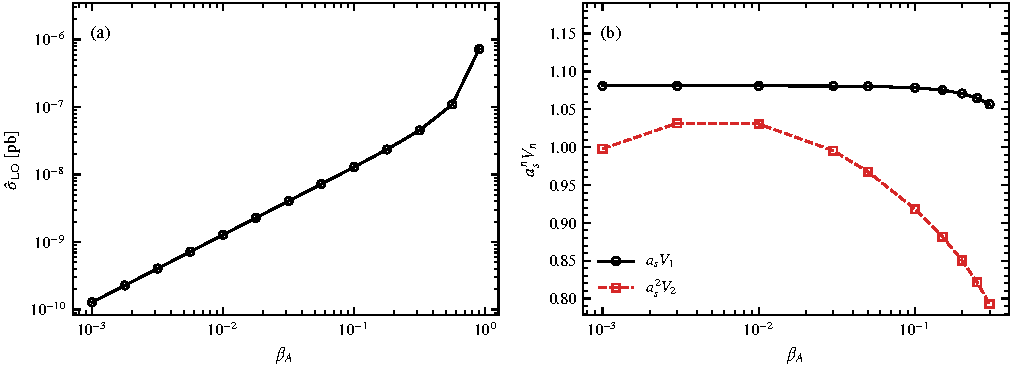
\includegraphics[width=0.94\textwidth]{figures/fig6_cross_section.pdf}
 \caption{(a) Leading order partonic cross section of the Type~II amplitude, Eq.~\eqref{eq:dsigma}, for $\mA=\BenchMA\,\mathrm{GeV}$, $\alpha_s=\BenchAlphaS$ and $\cot\beta_H=\BenchCotBeta$. (b) Finite virtual corrections of Eq.~\eqref{eq:virtual}, averaged over the angle, for $\muR=\mA$, $\Nc=\BenchNc$ and $\nf=\BenchNf$.}
 \label{fig:cross-section}
\end{figure*}

\subsection{Finite virtual corrections}

To examine the effect of the loop corrections on the Type~II squared amplitude, I define two dimensionless
coefficients, $V_1$ and $V_2$, relative to the tree contribution. Let $\mathcal A_{\Fin}$ denote the
amplitude constructed from the finite remainders of Eq.~\eqref{eq:catani}, in the normalisation of
Eq.~\eqref{eq:normalisation}. Using the helicity decomposition in Eq.~\eqref{eq:helicity}, its square
can be written as
\begin{align}
 \sum_{\mathrm{hel,col}}|\mathcal A_{\Fin}|^2
 &=2(\Nc^2-1)\,C_G^4
   \sum_i|\mathcal M_i^{(0)}|^2
 \nonumber\\
 &\quad\times
 \left[1+\as V_1+\as^2V_2+\Ord(\as^3)\right],
 \nonumber\\
 V_1
 &=\frac{
  2\Real\sum_i
  \mathcal M_i^{(0)*}\mathcal M_i^{(1)}
 }{
  \sum_i|\mathcal M_i^{(0)}|^2
 },
 \nonumber\\
 V_2
 &=\frac{
  \sum_i\left(
   2\Real\bigl[\mathcal M_i^{(0)*}\Mfull{i}\bigr]
   +|\mathcal M_i^{(1)}|^2
  \right)
 }{
  \sum_i|\mathcal M_i^{(0)}|^2
 }.
 \label{eq:virtual}
\end{align}
The sums run over the two tensor coefficients, $i=1,2$. The coefficient $V_1$ contains the
interference between the tree and one-loop amplitudes. At the next order, $V_2$ contains
both the interference between the tree and two-loop amplitudes and the square of the
one-loop amplitude.

These coefficients refer only to the $O_G$--$O_G$ Type~II contribution. Their
interpretation as NLO and NNLO finite virtual terms applies when the Type~II
tree amplitude is the leading amplitude, as for a pseudoscalar coupled to gluons
only through $G\tilde G$ (Sec.~\ref{sec:counting}). They do not
include interference with the Type~I amplitudes present in a 2HDM.

The quantities $V_1$ and $V_2$ depend on the subtraction scheme of
Eq.~\eqref{eq:catani}; they are not observables or $K$ factors. A physical
cross section requires the virtual and
real emission contributions to be combined consistently with the
counterterms for initial state collinear factorisation. The real
emission contributions are not included here.
%
At fixed $\bA$, both coefficients depend on the scattering angle. To display
their velocity dependence in Fig.~\ref{fig:cross-section}(b), I
average them over the angle using
the Type~II LO cross section as the weight:
\begin{equation}
 \langle V_n\rangle
 =
 \frac{
  \displaystyle
  \int_{-1}^{1}\dd c\,
  \sum_i|\mathcal M_i^{(0)}|^2\,V_n
 }{
  \displaystyle
  \int_{-1}^{1}\dd c\,
  \sum_i|\mathcal M_i^{(0)}|^2
 },
 \qquad n=1,2.
 \label{eq:angle-average}
\end{equation}
At fixed $\bA$, the remaining factors in Eq.~\eqref{eq:dsigma} are independent
of $c$ and cancel in this ratio. Thus, $\as\langle V_1\rangle$ and
$\as^2\langle V_2\rangle$ give the finite virtual contributions relative
to the angularly integrated tree contribution, rather than an
unweighted average of the corrections.
The integrals are evaluated with \QuadNodes-point Gauss--Legendre quadrature in $c$; with \QuadNodesRef{} points, $\langle V_1\rangle$ changes by less than \QuadVoneDev{} and $\langle V_2\rangle$ by less than \QuadVtwoDev{} relative to its value at $\bA=$ \QuadBetas{}.

I evaluate the one-loop remainders without a threshold expansion and
use the series through $\bA^6$ for the two-loop remainders.
For $\alpha_s=\BenchAlphaS$ and $\muR=\mA=\BenchMA\,\mathrm{GeV}$,
$\as\langle V_1\rangle$ lies between
\VoneMin{} and \VoneMax{}, while $\as^2\langle V_2\rangle$ lies between
\VtwoMin{} and \VtwoMax{} over $\VirtualBetaMin\leq\bA\leq\VirtualBetaMax$.
These are the two curves shown in
Fig.~\ref{fig:cross-section}(b).
At fixed kinematics, the scale dependence of the one-loop remainder
in Eq.~\eqref{eq:normalisation} implies $\partial V_1/\partial\ln\muR^2=4\beta_0$.

\paragraph{One-loop contribution.}

The threshold behaviour of $V_1$ and $V_2$ follows from the relative phases of the tree and loop
amplitudes. At fixed scattering angle, $\mathcal M_1^{(0)}\to2i\mA^2$, whereas
$\mathcal M_2^{(0)}$ vanishes as $\bA^2$.
The squared tree amplitude in the denominator of Eq.~\eqref{eq:virtual} therefore tends to
$4\mA^4$. At leading power, interference with the tree amplitude selects the imaginary part
of $\mathcal M_1^{(1)}$ or $\Mfull{1}$.

To separate the real logarithm from the constant phase, define
\[
 \ell=\ln\frac{2p_T}{\mA},
 \qquad
 \mathcal L=\ell+\frac{i\pi}{2}+\Ord(\bA^2),
\]
where the second relation follows from Eq.~\eqref{eq:calL}. At leading power, the
one-loop result in Eq.~\eqref{eq:one-loop-threshold} is
\[
 \frac{\mathcal M_1^{(1)}}{\mA^2}
 =
 \OneLoopAone\,\ell
 +\frac{i\pi}{2}\OneLoopAone
 +\widehat A^{(1)}_{10}.
\]
The coefficient of $\ell$ is real, so this term does not interfere with the imaginary
tree amplitude. The imaginary constant terms do contribute, giving
\begin{equation}
 V_1\longrightarrow
 \frac{\pi}{2}\OneLoopAone
 +\Imag\widehat A^{(1)}_{10}.
 \label{eq:v1-threshold}
\end{equation}
For $\Nc=\BenchNc$, $\nf=\BenchNf$ and
$\muR=\mA$, this gives
$V_1\to\VoneThreshold$.
Thus, the one-loop remainder contains a DPS logarithm, but the leading power
finite virtual correction does not. Its limiting value is independent of the
angle, which explains why the angular average in Fig.~\ref{fig:cross-section}(b)
is nearly constant.

\paragraph{Two-loop contribution.}

At the next order, the interference of the two-loop amplitude with the tree amplitude again selects the imaginary part of the loop remainder. The square of the one-loop amplitude, however,
retains the real logarithm. Using Eqs.~\eqref{eq:leading-power} and
\eqref{eq:one-loop-threshold}, the leading power terms of
Eq.~\eqref{eq:virtual} can be written as
\begin{align}
 V_2\big|_{\bA^0}
 &=
 \Imag\left[
  \sum_{k=0}^{3}\widehat A_{1k}\mathcal L^k
 \right] +
 \frac14\left|
  \OneLoopAone\,\mathcal L
  +\widehat A^{(1)}_{10}
 \right|^2
 +\frac{\pi^2\Nc^2}{16}.
\end{align}
The first term is the interference of the two-loop amplitude with the tree amplitude, and the second is the square of $\mathcal M_1^{(1)}$. The last term comes from $|\mathcal M_2^{(1)}|^2$,
since $\mathcal M_2^{(1)}\to\pi\Nc\mA^2/2$. It contributes at leading power even
though the corresponding tree amplitude vanishes. By contrast, interference
between $\mathcal M_2^{(0)}$ and $\Mfull{2}$ is suppressed by $\bA^2$,
up to logarithms.

The coefficients $\widehat A_{13}$ and $\widehat A_{12}$ are real. At leading power,
\[
 \Imag\mathcal L^3
 =\frac{3\pi}{2}\ell^2-\frac{\pi^3}{8},
 \qquad
 \Imag\mathcal L^2=\pi\ell.
\]
Consequently, the cubic logarithm of the two-loop amplitude gives a quadratic,
not a cubic, logarithm in its interference with the tree amplitude. The term
$\widehat A_{12}\mathcal L^2$ contributes only a linear logarithm to this
interference. The square of the one-loop amplitude is also at most
quadratic in $\ell$.

The leading threshold expansion of $V_2$ therefore has the form
\begin{equation}
 V_2=v_0+v_1\ell+v_2\ell^2
     +\Ord_{\log}(\bA^2).
 \label{eq:v2-form}
\end{equation}
Here $v_0$, $v_1$ and $v_2$ are the coefficients of the constant, linear
and quadratic terms in $\ell$. They all belong to the same
perturbative coefficient $V_2$; their subscripts do not count loops.

The coefficient $v_2$ receives two contributions.
The interference of the two-loop amplitude with the tree amplitude gives
$\tfrac32\pi\widehat A_{13}
=-14\pi^2\Nc^2$, while the square
of the one-loop amplitude gives
$\tfrac14(\OneLoopAone)^2
=\tfrac{49}{4}\pi^2\Nc^2$.
Their sum is
\begin{equation}
 v_2
 =-14\pi^2\Nc^2+\frac{49}{4}\pi^2\Nc^2
 =-\frac74\pi^2\Nc^2.
 \label{eq:v2-log}
\end{equation}
The two terms partly cancel, with the negative interference contribution
larger in magnitude. At leading power, the DPS logarithm thus first appears
in the finite virtual correction through $V_2$, where its highest
power is $\ell^2$.

A fit of the numerical values of $V_2$ at $c=\BenchCos$ over
$\VtwoBetaSmall\leq\bA\leq\VtwoBetaLarge$ gives $v_2=\VtwoLogFit$.
Equation~\eqref{eq:v2-log} gives $\VtwoLogExact$ for $\Nc=\BenchNc$;
the relative difference before rounding is \VtwoLogRelDiff{}. For $\as=\BenchAs$, the quadratic term
in the finite virtual correction is $\as^2v_2\ell^2=\VtwoLogScaled\,\ell^2$.

\paragraph{Remaining coefficients and numerical behaviour.}

At leading power, $v_0$, $v_1$ and $v_2$ are independent of the scattering
angle. The angular dependence of $V_2$ itself remains through $\ell$.
Fits for $v_0$ and $v_1$ at $c=0$, $\tfrac13$ and $\tfrac23$
agree within a relative spread of \VtwoAngleSpread{}.
The coefficient of the linear logarithm follows from the same expansion:
\begin{align*}
 v_1
 &=\pi\widehat A_{12}
   +\Imag\widehat A_{11}
   +\frac{\OneLoopAone}{2}
    \Real\widehat A^{(1)}_{10}
 \\
 &=\frac72\pi\Nc\Real\widehat A^{(1)}_{10}
   +7\pi^2\Nc\beta_0.
\end{align*}
For the benchmark parameters, this gives $v_1=\VoneFit$, in agreement with
the numerical fit to a relative difference of \VoneFormulaDev{}.
The coefficient is independent of $\muR$, since
$\Real\widehat A^{(1)}_{10}$ is scale independent. The same is true
of $v_2$. At leading power, the explicit scale dependence of $V_2$
is therefore confined to $v_0$, hich changes from \VzeroBench{}
to \VzeroTwoMu{} when $\muR$ is increased from $\mA$ to $2\mA$.

Although $\ell^2$ is the highest power of the logarithm, it need
not give the largest contribution at the velocities considered.
At $c=\BenchCos$, the ratio $(v_1\ell+v_2\ell^2)/V_2$ is
approximately \LogShareLarge\% at $\bA=\LogShareBetaLarge$
and \LogShareSmall\% at $\bA=\LogShareBetaSmall$.
The quadratic term alone contributes $-\SquareShareLarge\%$ and
$-\SquareShareSmall\%$ of the total $V_2$, respectively.
Since $\ell<0$ in this region and both $v_1$ and $v_2$ are
negative, the linear term is positive and the quadratic term is negative.
%
This competition also explains the shape of the correction as a
function of velocity. The leading power expression has a maximum at
\[
 \ell_{\mathrm{max}}
 =-\frac{v_1}{2v_2}
 =\VtwoPeakEll.
\]
At $c=\BenchCos$, this corresponds to $\bA\simeq\VtwoPeakBeta$.
For larger $\bA$, $\ell$ increases and the leading power value of
$V_2$ decreases. The same balance between the linear and quadratic
terms explains the turnover of the angular average
$\as^2\langle V_2\rangle$ in Fig.~\ref{fig:cross-section}(b).
At $c=\BenchCos$ and $\bA=\LogShareBetaLarge$,
including the terms beyond leading power changes $V_2$ by only \LeadPowerDevLarge\%.

\paragraph{DPS interpretation and subtraction dependence.}

The two contributions to $v_2$ also differ in their relation to the DPS
configuration. In the square of the one-loop amplitude, the DPS
region occurs in both the amplitude and its complex conjugate, that is,
on both sides of the final state cut. This is the configuration
associated with perturbative splittings in both protons that
overlaps with DPS and requires a subtraction to avoid double
counting~\cite{DiehlGauntSchoenwald2017,DiehlPloessl2026}.
In the interference with the tree amplitude, the DPS region occurs
only on the loop side of the cut. Both contributions enter the
finite virtual coefficient $V_2$ defined in Eq.~\eqref{eq:virtual}; the
logarithmic term in its one-loop square alone would therefore
not give the complete coefficient $v_2$.

Although $V_2$ depends on the IR subtraction convention, $v_2$ is unchanged by finite
scheme changes that multiply lower order amplitudes by angle independent functions
regular at the pair threshold. The tree amplitude has no
logarithm, and the one-loop remainder contains at most one power of $\ell$. Such changes can therefore
affect the constant and linear terms in $V_2$, but not the coefficient of $\ell^2$.

Finally, with the Wilson coefficient counting specified in
Sec.~\ref{sec:counting}, the one-loop $O_G$--$O_J$ amplitude contributes
at the same order as the two-loop $O_G$--$O_G$ amplitude.
Its coefficient $C_J$ depends on $m_t$ in the heavy top quark
theory~\cite{Bhattacharya:2019bmd}. By Eq.~\eqref{eq:gj-proportional},
the mixed amplitude is proportional to the tree amplitude. After
including its Wilson coefficient and matching the normalisation,
its interference with the tree amplitude therefore gives a
kinematically constant shift to $V_2$. It changes $v_0$,
but not $v_1$ or $v_2$, and is not included in the results above.


\subsection{Use in higher order calculations}
\label{sec:use}

The threshold series provide a compact representation of the two-loop Type~II finite remainders near the
pair production threshold. For the two-body virtual amplitude, $m_{AA}=\sqrt{\hat s}$, and
\[
 \frac{m_{AA}}{2\mA}
 =\frac{1}{\sqrt{1-\bA^2}}.
\]
The range $\bA\leq\RecommendedBeta$ therefore corresponds to pair invariant masses up to
$\ThresholdPercentPointTwo\%$ above $2\mA$. For $\mA=\BenchMA\,\mathrm{GeV}$, the upper limit
is $m_{AA}=\SqrtSPointTwo\,\mathrm{GeV}$. The point $\bA=\EdgeBeta$ lies
$\ThresholdPercentPointThree\%$ above threshold.

I recommend the series through $\bA^6$ for $0<\bA\leq\RecommendedBeta$ at the angles tested
in Tables~\ref{tab:validation-grid} and \ref{tab:forward-angles}.
At $\bA=\EdgeBeta$, the largest relative error
of the complete coefficients on the validation grid is \PtwoErrAtPointThree{}.
These numerical checks do not establish a uniform accuracy bound as $c\to\pm1$, where
the logarithms diverge. The series retain the complex values of both tensor coefficients,
including the phases needed for interference with other amplitudes. Such contributions
must be combined using the same normalisation, Wilson coefficient conventions, tensor basis
and infrared subtraction scheme.

One application is the calculation of the hard function for a threshold resummed or
soft-virtual prediction of the pair invariant mass distribution. In this context, threshold
refers to the limit in which little energy is available for additional QCD radiation
at fixed $m_{AA}$, rather than to the pair
production limit $\bA\to0$~\cite{Sterman:1986aj,Catani:1989ne,deFlorian:2015moa}.
At leading power in the soft limit, the soft and collinear factors are universal
for gluon fusion into a colour singlet final state. The process dependence enters
through the finite virtual contributions to the hard function~\cite{deFlorian:2012za,Bhattacharya:2021nsv}.
The hard function is therefore needed at each pair invariant mass, and the present
series provide its two-loop Type~II amplitude input near $m_{AA}=2\mA$.

To construct this contribution, the finite remainders must first be combined with
the appropriate lower order amplitudes. When the Type~II tree amplitude is the
leading amplitude, the relevant $O_G$--$O_G$ combinations are those in
Eq.~\eqref{eq:virtual}. In particular, the NNLO virtual term contains both the
interference of the two-loop amplitude with the tree amplitude and the square
of the one-loop amplitude. Integrated over the scattering angle at fixed $m_{AA}$ and
divided by the integrated tree contribution, they give the averages of
Eq.~\eqref{eq:angle-average}. The finite virtual terms must then
be combined with the universal contributions according to the
subtraction and resummation conventions of the chosen calculation~\cite{deFlorian:2012za}.
For Higgs pairs, Ref.~\cite{deFlorian:2015moa} gives an explicit construction in which
the two-loop finite virtual contribution is integrated over $t$ at fixed pair invariant mass.

The perturbative order of the present contribution depends on the leading
amplitude, as explained in Sec.~\ref{sec:counting}.
For a pseudoscalar coupled to gluons only through $G\tilde G$, the two-loop
Type~II remainders enter the NNLO virtual contribution. In a 2HDM, they first contribute at
N$^3$LO through interference with the leading Type~I amplitude.
In that case, the Type~II angular averages of Eq.~\eqref{eq:angle-average}
cannot be used directly: the interference with Type~I must be formed before the
angular integration. The remaining amplitudes and any mixed $O_G$--$O_J$ contribution must
also be included at the order required by the theory. For Higgs pairs, likewise,
the NNLO virtual corrections contain the diagrams with two effective vertices only
at tree level and at one loop~\cite{deFlorianMazzitelli2013Virtual},
and their two-loop terms are an ingredient of N$^3$LO~\cite{Banerjee:2018lfq}.
